\documentclass[spanish,]{article}
\usepackage{lmodern}
\usepackage{amssymb,amsmath}
\usepackage{ifxetex,ifluatex}
\usepackage{fixltx2e} % provides \textsubscript
\ifnum 0\ifxetex 1\fi\ifluatex 1\fi=0 % if pdftex
  \usepackage[T1]{fontenc}
  \usepackage[utf8]{inputenc}
\else % if luatex or xelatex
  \ifxetex
    \usepackage{mathspec}
  \else
    \usepackage{fontspec}
  \fi
  \defaultfontfeatures{Ligatures=TeX,Scale=MatchLowercase}
\fi
% use upquote if available, for straight quotes in verbatim environments
\IfFileExists{upquote.sty}{\usepackage{upquote}}{}
% use microtype if available
\IfFileExists{microtype.sty}{%
\usepackage{microtype}
\UseMicrotypeSet[protrusion]{basicmath} % disable protrusion for tt fonts
}{}
\usepackage[margin=1in]{geometry}
\usepackage{hyperref}
\hypersetup{unicode=true,
            pdfauthor={Alejandro Campoy Nieves; Gema Correa Fernández; Luis Gallego Quero; Jonathan Martín Valera; Andrea Morales Garzón},
            pdfborder={0 0 0},
            breaklinks=true}
\urlstyle{same}  % don't use monospace font for urls
\ifnum 0\ifxetex 1\fi\ifluatex 1\fi=0 % if pdftex
  \usepackage[shorthands=off,main=spanish]{babel}
\else
  \usepackage{polyglossia}
  \setmainlanguage[]{spanish}
\fi
\usepackage{color}
\usepackage{fancyvrb}
\newcommand{\VerbBar}{|}
\newcommand{\VERB}{\Verb[commandchars=\\\{\}]}
\DefineVerbatimEnvironment{Highlighting}{Verbatim}{commandchars=\\\{\}}
% Add ',fontsize=\small' for more characters per line
\usepackage{framed}
\definecolor{shadecolor}{RGB}{248,248,248}
\newenvironment{Shaded}{\begin{snugshade}}{\end{snugshade}}
\newcommand{\AlertTok}[1]{\textcolor[rgb]{0.94,0.16,0.16}{#1}}
\newcommand{\AnnotationTok}[1]{\textcolor[rgb]{0.56,0.35,0.01}{\textbf{\textit{#1}}}}
\newcommand{\AttributeTok}[1]{\textcolor[rgb]{0.77,0.63,0.00}{#1}}
\newcommand{\BaseNTok}[1]{\textcolor[rgb]{0.00,0.00,0.81}{#1}}
\newcommand{\BuiltInTok}[1]{#1}
\newcommand{\CharTok}[1]{\textcolor[rgb]{0.31,0.60,0.02}{#1}}
\newcommand{\CommentTok}[1]{\textcolor[rgb]{0.56,0.35,0.01}{\textit{#1}}}
\newcommand{\CommentVarTok}[1]{\textcolor[rgb]{0.56,0.35,0.01}{\textbf{\textit{#1}}}}
\newcommand{\ConstantTok}[1]{\textcolor[rgb]{0.00,0.00,0.00}{#1}}
\newcommand{\ControlFlowTok}[1]{\textcolor[rgb]{0.13,0.29,0.53}{\textbf{#1}}}
\newcommand{\DataTypeTok}[1]{\textcolor[rgb]{0.13,0.29,0.53}{#1}}
\newcommand{\DecValTok}[1]{\textcolor[rgb]{0.00,0.00,0.81}{#1}}
\newcommand{\DocumentationTok}[1]{\textcolor[rgb]{0.56,0.35,0.01}{\textbf{\textit{#1}}}}
\newcommand{\ErrorTok}[1]{\textcolor[rgb]{0.64,0.00,0.00}{\textbf{#1}}}
\newcommand{\ExtensionTok}[1]{#1}
\newcommand{\FloatTok}[1]{\textcolor[rgb]{0.00,0.00,0.81}{#1}}
\newcommand{\FunctionTok}[1]{\textcolor[rgb]{0.00,0.00,0.00}{#1}}
\newcommand{\ImportTok}[1]{#1}
\newcommand{\InformationTok}[1]{\textcolor[rgb]{0.56,0.35,0.01}{\textbf{\textit{#1}}}}
\newcommand{\KeywordTok}[1]{\textcolor[rgb]{0.13,0.29,0.53}{\textbf{#1}}}
\newcommand{\NormalTok}[1]{#1}
\newcommand{\OperatorTok}[1]{\textcolor[rgb]{0.81,0.36,0.00}{\textbf{#1}}}
\newcommand{\OtherTok}[1]{\textcolor[rgb]{0.56,0.35,0.01}{#1}}
\newcommand{\PreprocessorTok}[1]{\textcolor[rgb]{0.56,0.35,0.01}{\textit{#1}}}
\newcommand{\RegionMarkerTok}[1]{#1}
\newcommand{\SpecialCharTok}[1]{\textcolor[rgb]{0.00,0.00,0.00}{#1}}
\newcommand{\SpecialStringTok}[1]{\textcolor[rgb]{0.31,0.60,0.02}{#1}}
\newcommand{\StringTok}[1]{\textcolor[rgb]{0.31,0.60,0.02}{#1}}
\newcommand{\VariableTok}[1]{\textcolor[rgb]{0.00,0.00,0.00}{#1}}
\newcommand{\VerbatimStringTok}[1]{\textcolor[rgb]{0.31,0.60,0.02}{#1}}
\newcommand{\WarningTok}[1]{\textcolor[rgb]{0.56,0.35,0.01}{\textbf{\textit{#1}}}}
\usepackage{graphicx,grffile}
\makeatletter
\def\maxwidth{\ifdim\Gin@nat@width>\linewidth\linewidth\else\Gin@nat@width\fi}
\def\maxheight{\ifdim\Gin@nat@height>\textheight\textheight\else\Gin@nat@height\fi}
\makeatother
% Scale images if necessary, so that they will not overflow the page
% margins by default, and it is still possible to overwrite the defaults
% using explicit options in \includegraphics[width, height, ...]{}
\setkeys{Gin}{width=\maxwidth,height=\maxheight,keepaspectratio}
\IfFileExists{parskip.sty}{%
\usepackage{parskip}
}{% else
\setlength{\parindent}{0pt}
\setlength{\parskip}{6pt plus 2pt minus 1pt}
}
\setlength{\emergencystretch}{3em}  % prevent overfull lines
\providecommand{\tightlist}{%
  \setlength{\itemsep}{0pt}\setlength{\parskip}{0pt}}
\setcounter{secnumdepth}{0}
% Redefines (sub)paragraphs to behave more like sections
\ifx\paragraph\undefined\else
\let\oldparagraph\paragraph
\renewcommand{\paragraph}[1]{\oldparagraph{#1}\mbox{}}
\fi
\ifx\subparagraph\undefined\else
\let\oldsubparagraph\subparagraph
\renewcommand{\subparagraph}[1]{\oldsubparagraph{#1}\mbox{}}
\fi

%%% Use protect on footnotes to avoid problems with footnotes in titles
\let\rmarkdownfootnote\footnote%
\def\footnote{\protect\rmarkdownfootnote}

%%% Change title format to be more compact
\usepackage{titling}

% Create subtitle command for use in maketitle
\newcommand{\subtitle}[1]{
  \posttitle{
    \begin{center}\large#1\end{center}
    }
}

\setlength{\droptitle}{-2em}

  \title{}
    \pretitle{\vspace{\droptitle}}
  \posttitle{}
    \author{Alejandro Campoy Nieves \\ Gema Correa Fernández \\ Luis Gallego Quero \\ Jonathan Martín Valera \\ Andrea Morales Garzón}
    \preauthor{\centering\large\emph}
  \postauthor{\par}
      \predate{\centering\large\emph}
  \postdate{\par}
    \date{14 de noviembre de 2018}

\usepackage{fancyhdr}
\fancyfoot[CO,CE]{My footer}
\usepackage{color}
\usepackage{colortbl}
\usepackage{multicol}
\usepackage{multirow}

\begin{document}

\thispagestyle{empty}

\begin{center} \huge \textbf{Tratamiento Inteligente de datos} \end{center}
\vspace{0.3cm}
\begin{center} \huge \textbf{(TID)} \end{center}
\vspace{1.7cm}
\begin{center} \Large \textbf{\textsc{Prácticas de la asignatura}} \end{center}
\vspace{0.2cm}
\begin{center} \large \textbf{2018-2019} \end{center}

\vspace{2.5cm}

\textbf{\large En colaboración con:} \vspace{0.2cm}

\begin{figure}[h]
    \centering
    
\includegraphics[width=0.7\textwidth]{imagenes/logoUGR.jpg}
    \label{imagen2}
\end{figure}

\vspace{2.5cm}

\hspace{8.5cm}{\large \textbf{Participantes}}

\vspace{0.25cm}

\hspace{8.5cm}{Alejandro Campoy Nieves:  \href{mailto:alejandroac79@correo.ugr.es}{\textcolor{blue}{\underline{alejandroac79@correo.ugr.es}}}}

\vspace{0.15cm}

\hspace{8.5cm}{Gema Correa Fernández:  \href{mailto:gecorrea@correo.ugr.es}{\textcolor{blue}{\underline{gecorrea@correo.ugr.es}}} }

\vspace{0.15cm}

\hspace{8.5cm}{Luis Gallego Quero:  \href{mailto:lgaq94@correo.ugr.es}{\textcolor{blue}{\underline{lgaq94@correo.ugr.es}}} }

\vspace{0.15cm}

\hspace{8.5cm}{Jonathan Martín Valera:  \href{mailto:jmv742@correo.ugr.es}{\textcolor{blue}{\underline{jmv742@correo.ugr.es}}} }

\vspace{0.15cm}

\hspace{8.5cm}{Andrea Morales Garzón:  \href{mailto:andreamgmg@correo.ugr.es}{\textcolor{blue}{\underline{andreamgmg@correo.ugr.es}}} }

\vspace{0.15cm}

\newpage

\thispagestyle{empty}
\tableofcontents
\newpage

\thispagestyle{empty}
\listoffigures
\newpage

\thispagestyle{empty}
\listoftables
\newpage

\pagestyle{fancy}
\fancyhf{}
\lhead{Proyecto: Técnicas aplicadas para análisis inteligente de datos}
\rhead{\thepage}
\setcounter{page}{1}

\hypertarget{descripcion-de-los-paquetes-necesarios}{%
\section{Descripción de los paquetes
necesarios}\label{descripcion-de-los-paquetes-necesarios}}

A continuación, se describen los paquetes necesarios para el desarollo
del proyecto:

\begin{itemize}
\item
  \href{https://cran.r-project.org/web/packages/tm/tm.pdf}{\texttt{tm}}
  : Paquete específico para minería de datos, permite procesar datos de
  tipo texto. Se puede instalar usando :
  \emph{install.packages(``tm'')}.
\item
  \href{https://cran.r-project.org/web/packages/SnowballC/SnowballC.pdf}{\texttt{SnowballC}}
  : Paquete adicional para minería de datos, implementa un algoritmo que
  permite reducir el número de términos con lo que trabajar, es decir,
  agrupa aquellos términos que contienen la misma raíz. El paquete
  soporta los siguientes idiomas: alemán, danés, español, finlandés,
  francés, húngaro, inglés, italiano, noruego, portugués, rumano, ruso,
  sueco y turco. Se puede instalar usando :
  \emph{install.packages(``SnowballC'')}.
\item
  \href{https://cran.r-project.org/web/packages/wordcloud/wordcloud.pdf}{\texttt{wordcloud}}
  : Paquete para crear gráficas de nubes de palabras, permitiendo
  visualizar las diferencias y similitudes entre documentos. Se puede
  instalar usando : \emph{install.packages(``wordcloud'')}.
\item
  \href{https://cran.r-project.org/web/packages/arules/arules.pdf}{\texttt{arules}}
  : Paquete que proporciona la infraestructura para representar,
  manipular y analizar datos y patrones de transacción (conjuntos de
  elementos frecuentes y reglas de asociación). Se puede instalar usando
  : \emph{install.packages(``arules'')}.
\item
  \href{https://cran.r-project.org/web/packages/arulesViz/arulesViz.pdf}{\texttt{arulesViz}}
  : Paquete que extiende el paquete `arules' con varias técnicas de
  visualización para reglas de asociación y conjuntos de elementos. El
  paquete también incluye varias visualizaciones interactivas para la
  exploración de reglas. Se puede instalar usando :
  \emph{install.packages(``arulesViz'')}.
\end{itemize}

\newpage

\hypertarget{comprender-el-problema-a-resolver}{%
\section{1. Comprender el problema a
resolver}\label{comprender-el-problema-a-resolver}}

Para la realización y aplicación de las técnicas explicadas a lo largo
del curso, se ha seleccionado el \emph{dataset}
\href{https://archive.ics.uci.edu/ml/datasets/Drug+Review+Dataset+\%28Druglib.com\%29}{\textbf{Drug
Review Dataset}}, proporcionado por
\href{https://archive.ics.uci.edu/ml/index.php}{\emph{UCI Machine
Learning Repository}}. Dicho \emph{dataset} contiene una exhaustiva base
de datos de medicamentos específicos, en donde, el conjunto de datos
proporciona revisiones de pacientes sobre medicamentos específicos para
unas condiciones particulares. Las revisiones se encuentran desglosadas
en función del tema que se esté tratando : beneficios, efectos
secundarios y comentarios generales. De igual modo, se dispone de una
calificación de satisfacción general, es decir, una calificación en base
a los efectos secundarios y otra a la efectividad del medicamento.

En este proyecto nos centraremos en el \textbf{análisis y experiencia de
los usuarios}, obtenido mediante la ingesta de ciertos medicamentos.
Para ello, se proponen los siguientes objetivos principales del estudio:

\begin{itemize}
\item
  Realizar un análisis de sentimientos en relación con la experiencia en
  el uso de dichos medicamentos, como por ejemplo ver la efectividad del
  medicamento con los efectos secundarios o beneficios del mismo.
\item
  Compatibilizar dicho modelo de datos con otros conjuntos de datos
  aportados en \href{https://www.drugs.com/}{\textbf{Drugs.com}}.
\end{itemize}

Las características de este conjunto de datos vienen descritas en la
siguiente tabla:

\begin{table}[h]
    \begin{center}
        \begin{tabular}{|>{\columncolor[rgb]{0.94,0.97,1.0}}l|c|}
            \hline 
            \textbf{Características del Data Set} & Multivariable, texto \\ \hline
            \textbf{Características de los atributos} & Discreto, texto \\ \hline
            \textbf{Tareas asociadas} & Clasificación, regresión, Clustering \\ \hline
            \textbf{Número de instancias} & 4143 \\ \hline
            \textbf{Número de atributos} & 8 \\ \hline
            \textbf{Valores vacíos} & N/A \\ \hline
            \textbf{Área} & N/A \\ \hline
            \textbf{Fecha de donación} & 10/02/2018 \\ \hline
            \textbf{Veces visualizado} & 9130 \\ \hline
        \end{tabular}
        \caption{Relevancia de requisitos para preselección de candidatos.}
        \label{tabla:preseleccion}
    \end{center}
\end{table}

Los datos se dividen en un conjunto train (75\%) y otro conjunto test
(25\%) y se almacenan en dos archivos.tsv (tab-separated-values),
respectivamente. Los atributos que tenemos en este dataset son:

\begin{enumerate}
\def\labelenumi{\arabic{enumi}.}
\tightlist
\item
  \textbf{urlDrugName} (categorical): nombre del medicamento
\item
  \textbf{rating} (numerical): clasificación de 1 a 10 del medicamento
  según el paciente
\item
  \textbf{effectiveness} (categorical): clasificación de la efectividad
  del medicamento según el paciente (5 posibles valores)
\item
  \textbf{sideEffects} (categorical): clasificación de los efectos
  secundarios del medicamento según el paciente (5 posibles valores)
\item
  \textbf{condition} (categorical): nombre de la condición (diagnóstico)
\item
  \textbf{benefitsReview} (text): opinión del paciente sobre los
  beneficios
\item
  \textbf{sideEffectsReview} (text): opinión del paciente sobre los
  efectos secundarios
\item
  \textbf{commentsReview} (text): comentario general del paciente
\end{enumerate}

\hypertarget{preprocesamiento-de-datos}{%
\section{2. Preprocesamiento de datos}\label{preprocesamiento-de-datos}}

En este apartado, pondremos los datos a puntos para la aplicación de
técnicas. Para poder analizar el \emph{dataset} y realizar el
preprocesamiento al mismo, lo primero que se va hacer es leer el
conjunto de datos \emph{train} y \emph{test}.

\hypertarget{lectura-de-datos}{%
\subsection{2.1. Lectura de datos}\label{lectura-de-datos}}

\begin{Shaded}
\begin{Highlighting}[]
\CommentTok{# Lectura de datos train}
\NormalTok{datos_train <-}\StringTok{ }\KeywordTok{read.table}\NormalTok{(}\StringTok{"datos/drugLibTrain_raw.tsv"}\NormalTok{, }\DataTypeTok{sep=}\StringTok{"}\CharTok{\textbackslash{}t}\StringTok{"}\NormalTok{, }\DataTypeTok{comment.char=}\StringTok{""}\NormalTok{,}
                          \DataTypeTok{quote =} \StringTok{"}\CharTok{\textbackslash{}"}\StringTok{"}\NormalTok{, }\DataTypeTok{header=}\OtherTok{TRUE}\NormalTok{)}
\end{Highlighting}
\end{Shaded}

\begin{Shaded}
\begin{Highlighting}[]
\CommentTok{# Visualizar las 5 primeras filas para los datos train}
\KeywordTok{head}\NormalTok{(datos_train, }\DecValTok{5}\NormalTok{) }
\end{Highlighting}
\end{Shaded}

\begin{verbatim}
##      X      urlDrugName rating        effectiveness         sideEffects
## 1 2202        enalapril      4     Highly Effective   Mild Side Effects
## 2 3117 ortho-tri-cyclen      1     Highly Effective Severe Side Effects
## 3 1146          ponstel     10     Highly Effective     No Side Effects
## 4 3947         prilosec      3 Marginally Effective   Mild Side Effects
## 5 1951           lyrica      2 Marginally Effective Severe Side Effects
##                                condition
## 1 management of congestive heart failure
## 2                       birth prevention
## 3                       menstrual cramps
## 4                            acid reflux
## 5                           fibromyalgia
##                                                                                                                                                                                                                                                                                                                                                                                                                                                                                                                                                                                                           benefitsReview
## 1                                                                                                                                                                                                                                                                                                                                                                                                                         slowed the progression of left ventricular dysfunction into overt heart failure \n\n\nalone or with other agents in the managment of hypertension \n\n\nmangagement of congestive heart failur
## 2                                                                                                                                                                                                                                                                                                                                                                                                                                     Although this type of birth control has more cons than pros, it did help with my cramps. It's also effective with the prevention of pregnancy. (Along with use of condoms as well)
## 3                                                                                                                                                                                                                                                                                                                                                         I was used to having cramps so badly that they would leave me balled up in bed for at least 2 days.  The Ponstel doesn't take the pain away completely, but takes the edge off so much that normal activities were possible. Definitely a miracle medication!!
## 4 The acid reflux went away for a few months after just a few days of being on the drug. The heartburn started again as soon as I stopped taking it. So I began treatment again. 6 months passed and I stopped taking it. The heartburn came back, and seemed worse even. The doctor said I should try another 6 month treatment. I did, and the same exact thing happened. This went on for about three years. I asked why this wasn't curing my reflux. The doctor quite frankly told me that it wasn't a cure, but a "treatment for the symptoms". I was told that I would probably be on it for the rest of my life.
## 5                                                                                                                                                                                                                                                                                                                                                                                                                                                                                                     I think that the Lyrica was starting to help with the pain, but the side-effects were just too severe to continue.
##                                                                                                                                                                                                                                                    sideEffectsReview
## 1                                                              cough, hypotension , proteinuria, impotence , renal failure , angina pectoris , tachycardia , eosinophilic pneumonitis, tastes disturbances , anusease anorecia , weakness fatigue insominca weakness
## 2 Heavy Cycle, Cramps, Hot Flashes, Fatigue, Long Lasting Cycles. It's only been 5 1/2 months, but i'm concidering changing to a different bc. This is my first time using any kind of bc, unfortunately due to the constant hassel, i'm not happy with the results.
## 3                                                                                                                                                                                                                         Heavier bleeding and clotting than normal.
## 4                                                                                                                                                    Constipation, dry mouth and some mild dizziness that would go away after medication was stopped for a few days.
## 5                                                                                                             I felt extremely drugged and dopey.  Could not drive at all while on this med.  Also had extreme ankle and feet swelling and couldn't even wear shoes.
##                                                                                                                                                                                                                                                                                                                                                                                        commentsReview
## 1                                                                                                                                                                                                                                                                                                                                   monitor blood pressure , weight and asses for resolution of fluid
## 2                                                                                                                                                                                                                                                                                                                                      I Hate This Birth Control, I Would Not Suggest This To Anyone.
## 3 I took 2 pills at the onset of my menstrual cramps and then every 8-12 hours took 1 pill as needed for about 3-4 days until cramps were over. If cramps are bad, make sure to take every 8 hours on the dot because the medication stops working suddenly and unfortunately takes about an hour to an hour and a half to kick back in.. if cramps are only moderate, taking every 12 hours is okay.
## 4                                                                                                                                                                                                                                      I was given Prilosec prescription at a dose of 45mg per day. Medication was taken once, every morning before eating. Each treatment duration was for 6 months.
## 5                                                                                                                                                                                                                                                                                                                                                                                           See above
\end{verbatim}

\begin{Shaded}
\begin{Highlighting}[]
\CommentTok{# Resumen sobre los datos train}
\KeywordTok{summary}\NormalTok{(datos_train) }
\end{Highlighting}
\end{Shaded}

\begin{verbatim}
##        X          urlDrugName       rating      
##  Min.   :   0   lexapro :  63   Min.   : 1.000  
##  1st Qu.:1062   prozac  :  46   1st Qu.: 5.000  
##  Median :2092   retin-a :  45   Median : 8.000  
##  Mean   :2081   zoloft  :  45   Mean   : 7.006  
##  3rd Qu.:3092   paxil   :  38   3rd Qu.: 9.000  
##  Max.   :4161   propecia:  38   Max.   :10.000  
##                 (Other) :2832                   
##                 effectiveness                         sideEffects  
##  Considerably Effective: 928   Extremely Severe Side Effects: 175  
##  Highly Effective      :1330   Mild Side Effects            :1019  
##  Ineffective           : 247   Moderate Side Effects        : 614  
##  Marginally Effective  : 187   No Side Effects              : 930  
##  Moderately Effective  : 415   Severe Side Effects          : 369  
##                                                                    
##                                                                    
##                condition   
##  depression         : 236  
##  acne               : 165  
##  anxiety            :  63  
##  insomnia           :  54  
##  birth control      :  49  
##  high blood pressure:  42  
##  (Other)            :2498  
##                                                                                                                                                                                                                                                                                                                          benefitsReview
##  none                                                                                                                                                                                                                                                                                                                           :  20  
##  None                                                                                                                                                                                                                                                                                                                           :  18  
##  NONE                                                                                                                                                                                                                                                                                                                           :   3  
##  None.                                                                                                                                                                                                                                                                                                                          :   3  
##  The treatment benefits were marginal at best.  Mood neither improved nor deteriorated, and anxiety was never significantly alleviated.  Unsurprisingly, recent research suggests that SSRIs are only effective in the most severe of cases.                                                                                    :   3  
##  Before the use of vagifem tablets, I had to endure a series of urinary infections after sometimes painful sexual intercourse.  I also had painful cracks in mucoal lining of vulva due to aging and dryness.  After beginning the use of this drug, I found that the ncreased mucous in vagina resolved both of these problems.:   2  
##  (Other)                                                                                                                                                                                                                                                                                                                        :3058  
##                    sideEffectsReview               commentsReview
##  none                       : 112    n/a                  :   7  
##  None                       :  73    none                 :   6  
##  None.                      :  19    None                 :   4  
##  No side effects.           :   9    .                    :   3  
##  There were no side effects.:   6    One tablet once a day:   3  
##  no side effects            :   5    (Other)              :3083  
##  (Other)                    :2883    NA's                 :   1
\end{verbatim}

\begin{Shaded}
\begin{Highlighting}[]
\CommentTok{# Lectura de datos test}
\NormalTok{datos_test <-}\StringTok{ }\KeywordTok{read.table}\NormalTok{(}\StringTok{"./datos/drugLibTest_raw.tsv"}\NormalTok{, }\DataTypeTok{sep=}\StringTok{"}\CharTok{\textbackslash{}t}\StringTok{"}\NormalTok{, }\DataTypeTok{comment.char=}\StringTok{""}\NormalTok{,}
                         \DataTypeTok{quote =} \StringTok{"}\CharTok{\textbackslash{}"}\StringTok{"}\NormalTok{, }\DataTypeTok{header=}\OtherTok{TRUE}\NormalTok{)}
\end{Highlighting}
\end{Shaded}

\begin{Shaded}
\begin{Highlighting}[]
\CommentTok{# Visualizar las 5 primeras filas para los datos test}
\KeywordTok{head}\NormalTok{(datos_test, }\DecValTok{5}\NormalTok{) }
\end{Highlighting}
\end{Shaded}

\begin{verbatim}
##      X urlDrugName rating          effectiveness         sideEffects
## 1 1366      biaxin      9 Considerably Effective   Mild Side Effects
## 2 3724    lamictal      9       Highly Effective   Mild Side Effects
## 3 3824    depakene      4   Moderately Effective Severe Side Effects
## 4  969     sarafem     10       Highly Effective     No Side Effects
## 5  696    accutane     10       Highly Effective   Mild Side Effects
##            condition
## 1    sinus infection
## 2   bipolar disorder
## 3   bipolar disorder
## 4 bi-polar / anxiety
## 5       nodular acne
##                                                                                                                                                                                                                                                                                                                                                                                                                                                                                                                                                                                                                                                                                                                                                                                                                                                                                                                                        benefitsReview
## 1                                                                                                                                                                                                                                                                                                                                                                                                                                                                                                                                                                                                                                                                                                                                                                                                            The antibiotic may have destroyed bacteria causing my sinus infection.  But it may also have been caused by a virus, so its hard to say.
## 2 Lamictal stabilized my serious mood swings. One minute I was clawing up the walls in pure mania, the next curled up in a fetal position on my bed contemplating suicdie. I am no longer at the whim of my moods and neither are those around me. I'm lucky that I started pharmaceuticals almost immediately after I was diagnosed a bipolar. Lamictal gives me amazing clarity to go about my day, honestly assess myself and form real relationships. Lamitcal lifted a fog, I guess you could call it. Now that I'm medicated I realize how cloudy my thought processes used to be. It's a wonderful feeling.\n\n\n\n\n\nInterestingly, I hardly dreamt before beginning Lamictal. I would dream (I mean dream in the sense of being able to imagine pictures and scenes while asleep, not REM) maybe once every two months. Now I dream every night. I found that the closer I take it to bedtime the more frequent and more intense my dreams.
## 3                                                                                                                                                                                                                                                                                                                       Initial benefits were comparable to the brand name version of this drug, Depakote.  I had been taking Depakote for several months and experienced great results.  When I went to my psychiatrist for an evaluation and re-fill, he accidently prescribed the generic version, Depakene.  When I discovered the error, I was told by this doctor that I would experience the same results as Depakote.  The positive side effects of the Depakene: balanced mood, improved concentration, improved logical cognition, mental clarity, lessened anxiety and irritability, improved sleep, increase in pleasure about activities
## 4                                                                                                                                                                                                                                                                                                                                                                                                                                                                                                                                                                                                                                                                                                    It controlls my mood swings. It helps me think before i act or speak. It controlls amxiety. IT FREED ME TO LIVE MY LIFE HAPPILY!!! I cared about my life more. Everything had more meaning to me. I lived a very dull life before taking prozac.
## 5                                                                                                                                                                                                                                                                                                                                                                                                                                                                                                                                                                        Within one week of treatment superficial acne lesions were visibly reduced.  Sebum production which had been excessive before beginning was significantly reduced (after course of treatment level increased to a more normal level).  After one month of treatment no new acne lesions occured.  By the end of treatment no new acne developed, and old lesions had healed.
##                                                                                                                                                                                                                                                                                                                                                                                                                                                                                                                                                                                                                                                                                                                                                                                                                                                                                                                                                                                             sideEffectsReview
## 1                                                                                                                                                                                                                                                                                                                                                                                                                                                                                                                                                                                                                                                                                                                                                                                                                                                                                                                                                                               Some back pain, some nauseau.
## 2 Drowsiness, a bit of mental numbness. If you take too much, you will feel sedated. Since you have to be able to clearly and honestly assess your emotions and thoughts, determining how much medication you need is tough. I found that 400mg works perfectly for me, but that's a high dose. Less than that and I can feel the medicine wearing off prematurely (I like it to last 24hrs, from sleep to sleep). More than that and I feel numb. Some might call it drowsiness, but it's more a sluggishness of the mind for me.\n\n\n\n\n\nBefore I began treating my bipolar disorder, I used to write a fair amount of fiction. It sort of flowed from me. I definitely had the artist's temperament. After Lamictal, though, that inherent creativity fizzled out. It doesn't come spilling out of me while I'm deep into a manic euphoria. I have to work at art now. It's something that requires discipline. If you are in a field which requires creativity, expect to see a change in your output.
## 3                                                                                                                                                                                                                                                                                                             Depakene has a very thin coating, which caused severe heart burn and stomach upset.  The discomfort was so unpleasant that it made me not want to take my meds, so I was not taking them consistently as prescribed.  This caused my mood to fluctuate again.  Even after I switched to the Depakote, my stomach was still uncomfortable for several weeks afterwards.  My appetite decreased and food was very unappetizing.  Certain foods that I normally enjoy, such as chicken or fish, made me feel extremely queasy when I ate them.  I did not like the physical side effect of the drug, and decided to quit my psychiatric drugs altogether - because I was no longer stable anymore!
## 4                                                                                                                                                                                                                                                                                                                                                                                                                                                                                                                                                                                                                                                                                                                                                                                                                                                                                                                                                                     I didnt really notice any side effects.
## 5                                                                                                                                                                                                                                                                                                                                                                                                                                                                                                                                                                                                                                                                                                                                                                                                                                                                      Side effects included moderate to severe dry skin.  This condition was rectified by the topical application of "Aquafore" moisturizer.
##                                                                                                                                                                                                                                                                                                                                                                                                                                                                                                                                                                                                                                                                                                                                                                                                                                                                                                                                                                                                                                                                                                                                                                                                                                      commentsReview
## 1                                                                                                                                                                                                                                                                                                                                                                                                                                                                                                                                                                                                                                                                                                                                                                                                                                                                                                                                                                                                                                                                                                                                                                     Took the antibiotics for 14 days. Sinus infection was gone after the 6th day.
## 2                                                                                                                                                                                                                                                                                                                                                                                                                                                                                                                                                                                                                                                                                                                                                                                                                                                                                                                Severe mood swings between hypomania and depression with suicide ideation before Lamictal. Began with 10mg and tritrated up to 400mg over a few months. Played around with the dosage to finally arrive at 400mg. Experimented with taking it at different times in the evening. Found that most comfortable time is before sleep.
## 3 Depakote was prescribed to me by a Kaiser psychiatrist in Pleasant Hill, CA in 2006.  The medication was given to help treat the diagnosis of Bipolar Disorder, Type II.  My disease was misdiagnosed for several years as depression, since I was never seen by a professional during hypomanic episodes, and when I did see a professional, I did not think that my manic symptoms were signs of a serious psychiatric problem.  Anti-depressant drugs were prescribed: Prozac in 2001, which had minimal effect and I stopped taking them a few months later. Wellbutrin was prescribed again for "chronic depression" in the spring of 2006, but this medication slowly spun me into an intense manic period.  After the manic episode, I fell very hard into a severe, suicidal depressive state.  I was voluntarily admitted to a psychiatric ward in June 2006 to keep me safe and to properly diagnose my condition.  The symptoms I was experiencing before being prescribed the Depakote/Depakene: rapidly cycling mood swings between intense activation and irritablity/excitement and crashing lows and depression, suicidal thoughts, poor logic and decision making, racing thoughts, anxiety, poor concentration, and poor sleep.
## 4                                                                                                                                                                                                                                                                                                                                                                                                                                                                                                                                                                                                                                                                                                                                                                                                                                                                                                                                                                                                                                                                                                                              This drug may not be for everyone but its wonderful for me! It makes me a totally different person, a better person.
## 5                                                                                                                                                                                                                                                                                                                                                                                                                                                                                                                                                                                                                                                                                                                                                                                                                                                                                                                                                                                                                                 Drug was taken in gelatin tablet at 0.5 mg per day.  Drug treatment was carried out with bi-monthly visits to physician.  After 25 weeks ended treatment successfully finished treatment.  No recurrence of acne.
\end{verbatim}

\begin{Shaded}
\begin{Highlighting}[]
\CommentTok{# información sobre los datos test}
\KeywordTok{summary}\NormalTok{(datos_test) }
\end{Highlighting}
\end{Shaded}

\begin{verbatim}
##        X              urlDrugName      rating      
##  Min.   :   1.0   paxil     : 20   Min.   : 1.000  
##  1st Qu.: 968.2   effexor-xr: 17   1st Qu.: 5.000  
##  Median :2048.0   accutane  : 16   Median : 8.000  
##  Mean   :2085.4   synthroid : 15   Mean   : 6.767  
##  3rd Qu.:3199.8   differin  : 13   3rd Qu.: 9.000  
##  Max.   :4157.0   effexor   : 13   Max.   :10.000  
##                   (Other)   :942                   
##                 effectiveness                        sideEffects 
##  Considerably Effective:310   Extremely Severe Side Effects: 80  
##  Highly Effective      :411   Mild Side Effects            :330  
##  Ineffective           : 82   Moderate Side Effects        :236  
##  Marginally Effective  : 76   No Side Effects              :268  
##  Moderately Effective  :157   Severe Side Effects          :122  
##                                                                  
##                                                                  
##                condition  
##  depression         : 66  
##  acne               : 46  
##  anxiety            : 27  
##  insomnia           : 21  
##  high blood pressure: 20  
##  birth control      : 19  
##  (Other)            :837  
##                                                                                                                                                                                                                                                                                                                benefitsReview
##  none                                                                                                                                                                                                                                                                                                                 :   6  
##  None                                                                                                                                                                                                                                                                                                                 :   5  
##  elevation of mood and clarity of thought.  Progress stalled out at 300 mg, but with increase to 450 mg can tell the difference.  I'm able to finally think and plan ahead and chip away at all the clutter I've not been able to deal with which accumulated while depressed.                                        :   3  
##  I've only been on it for a week but I've noticed a change already. I am more awake and it seems as though a fog has been lifted. I am thinking more clearly and don't feel so down.                                                                                                                                  :   2  
##  The benefits of using Tretinoin were great. First of all I noticed that my skin started glowing and my acne diminished greatly. But I had to be very patient because the results were not immediate. Continued use of the medicine rendered amazing results. My skin is a lot more smoother, healthier, and brighter.:   2  
##  !0 years after spinal stenosis, scar-tissue and additional narrowing of nerve canals causes sever inflammation and pain. My back pain is virtually disappeared, I feel like a new kid on the block                                                                                                                   :   1  
##  (Other)                                                                                                                                                                                                                                                                                                              :1017  
##                                                                                                                                                                                                                                                                                                                                                                                                             sideEffectsReview
##  none                                                                                                                                                                                                                                                                                                                                                                                                                : 29    
##  None                                                                                                                                                                                                                                                                                                                                                                                                                : 23    
##  None.                                                                                                                                                                                                                                                                                                                                                                                                               : 11    
##  none at 300 mg.  Possible tinnitus from increase to 450 mg, not evaluated by an audiologist yet though.  Did experience weight loss (7 lbs.) at 450 mg dosage.                                                                                                                                                                                                                                                      :  3    
##  dryness                                                                                                                                                                                                                                                                                                                                                                                                             :  2    
##  luckily I did not notice any negative side effects. The positive effects that I noticed out weighed the negative ones. The side effects that i noticed were very slight peeling of the skin and a very very slight burning sensation. The burning sensation however, completely went away with continued use of the medicine. I believe this is so because my skin became more and more tolerant the more I used it.:  2    
##  (Other)                                                                                                                                                                                                                                                                                                                                                                                                             :966    
##                                                                                                                                                                                                                                                                                                                                                                                                                                                                                                                       commentsReview
##  Initial treatment included therapy and Lexapro in addition to Wellbutrin XL.  Now only on the Wellbutrin XL.  I see the psychiatrist every 4 months for re-evaluation.                                                                                                                                                                                                                                                                                                                                                      :   3  
##  My doctor added Abilify to my 60 mg of Cymbalta because I was feeling really fatigued and unable to function.                                                                                                                                                                                                                                                                                                                                                                                                               :   2  
##  My treatment details are as follows: I Used Avita (Tretinoin) every night after cleansing my face. I waited about 15-20 minutes after cleansing to apply a dime size of the medication. My doctor recommended doing so to make the skin less sensitive and more receptive of the drug. My doctor also told me that the use of sunscreen was imperative while using Tretinoin because retinol can cause the skin to become sensitive to sunlight. So every morning before leaving the house I made sure to apply a sunscreen.:   2  
##  none                                                                                                                                                                                                                                                                                                                                                                                                                                                                                                                        :   2  
##  see above                                                                                                                                                                                                                                                                                                                                                                                                                                                                                                                   :   2  
##  ?                                                                                                                                                                                                                                                                                                                                                                                                                                                                                                                           :   1  
##  (Other)                                                                                                                                                                                                                                                                                                                                                                                                                                                                                                                     :1024
\end{verbatim}

\begin{Shaded}
\begin{Highlighting}[]
\KeywordTok{View}\NormalTok{(datos_train)    }\CommentTok{# vista de la tabla}
\KeywordTok{View}\NormalTok{(datos_test)    }\CommentTok{# vista de la tabla}
\end{Highlighting}
\end{Shaded}

\hypertarget{procesar-datos}{%
\subsection{2.2. Procesar datos}\label{procesar-datos}}

\hypertarget{cuantificacion-de-variables}{%
\subsubsection{2.2.1. Cuantificación de
variables}\label{cuantificacion-de-variables}}

Para poder analizar y trabajar más fácilmente con la información de
\emph{sideEffects} y \emph{effectiveness}, vamos a realizar una
conversión de dichas columnas a forma cuantitativa.

A continuación vamos a cuantificar la columna de \emph{sideEffects},
añadiendo una nueva columna a nuestro conjunto de datos llamada
\emph{sideEffectsNumber} que nos clasifica los posibles valores de la
columna sideEffects en un rango numérico. Este rango está comprendido
entre 1 y 5, asignando los siguientes valores:

\begin{Shaded}
\begin{Highlighting}[]
\CommentTok{# Datos de entrenamiento}
\NormalTok{datos_train}\OperatorTok{$}\NormalTok{sideEffectsNumber[datos_train}\OperatorTok{$}\NormalTok{sideEffects }\OperatorTok{==}\StringTok{ "Extremely Severe Side Effects"}\NormalTok{] <-}\StringTok{ }\DecValTok{5}
\NormalTok{datos_train}\OperatorTok{$}\NormalTok{sideEffectsNumber[datos_train}\OperatorTok{$}\NormalTok{sideEffects }\OperatorTok{==}\StringTok{ "Severe Side Effects"}\NormalTok{] <-}\StringTok{ }\DecValTok{4}
\NormalTok{datos_train}\OperatorTok{$}\NormalTok{sideEffectsNumber[datos_train}\OperatorTok{$}\NormalTok{sideEffects }\OperatorTok{==}\StringTok{ "Moderate Side Effects"}\NormalTok{] <-}\StringTok{ }\DecValTok{3}
\NormalTok{datos_train}\OperatorTok{$}\NormalTok{sideEffectsNumber[datos_train}\OperatorTok{$}\NormalTok{sideEffects }\OperatorTok{==}\StringTok{ "Mild Side Effects"}\NormalTok{] <-}\StringTok{ }\DecValTok{2}
\NormalTok{datos_train}\OperatorTok{$}\NormalTok{sideEffectsNumber[datos_train}\OperatorTok{$}\NormalTok{sideEffects }\OperatorTok{==}\StringTok{ "No Side Effects"}\NormalTok{] <-}\StringTok{ }\DecValTok{1}

\CommentTok{# Datos de test}
\NormalTok{datos_test}\OperatorTok{$}\NormalTok{sideEffectsNumber[datos_test}\OperatorTok{$}\NormalTok{sideEffects }\OperatorTok{==}\StringTok{ "Extremely Severe Side Effects"}\NormalTok{] <-}\StringTok{ }\DecValTok{5}
\NormalTok{datos_test}\OperatorTok{$}\NormalTok{sideEffectsNumber[datos_test}\OperatorTok{$}\NormalTok{sideEffects }\OperatorTok{==}\StringTok{ "Severe Side Effects"}\NormalTok{] <-}\StringTok{ }\DecValTok{4}
\NormalTok{datos_test}\OperatorTok{$}\NormalTok{sideEffectsNumber[datos_test}\OperatorTok{$}\NormalTok{sideEffects }\OperatorTok{==}\StringTok{ "Moderate Side Effects"}\NormalTok{] <-}\StringTok{ }\DecValTok{3}
\NormalTok{datos_test}\OperatorTok{$}\NormalTok{sideEffectsNumber[datos_test}\OperatorTok{$}\NormalTok{sideEffects }\OperatorTok{==}\StringTok{ "Mild Side Effects"}\NormalTok{] <-}\StringTok{ }\DecValTok{2}
\NormalTok{datos_test}\OperatorTok{$}\NormalTok{sideEffectsNumber[datos_test}\OperatorTok{$}\NormalTok{sideEffects }\OperatorTok{==}\StringTok{ "No Side Effects"}\NormalTok{] <-}\StringTok{ }\DecValTok{1}
\end{Highlighting}
\end{Shaded}

Podemos comprobar que se ha creado la nueva columna
\emph{sideEffectsNumber}, y que se han añadido los nuevos cambios.

\begin{Shaded}
\begin{Highlighting}[]
\KeywordTok{head}\NormalTok{(datos_train}\OperatorTok{$}\NormalTok{sideEffectsNumber, }\DecValTok{10}\NormalTok{) }
\end{Highlighting}
\end{Shaded}

\begin{verbatim}
##  [1] 2 4 1 2 4 4 2 1 1 5
\end{verbatim}

Volvemos a aplicar el mismo proceso para la columna de
\emph{effectiveness}.

\begin{Shaded}
\begin{Highlighting}[]
\CommentTok{# Datos de entrenamiento}
\NormalTok{datos_train}\OperatorTok{$}\NormalTok{effectivenessNumber[datos_train}\OperatorTok{$}\NormalTok{effectiveness }\OperatorTok{==}\StringTok{ "Highly Effective"}\NormalTok{] <-}\StringTok{ }\DecValTok{5}
\NormalTok{datos_train}\OperatorTok{$}\NormalTok{effectivenessNumber[datos_train}\OperatorTok{$}\NormalTok{effectiveness }\OperatorTok{==}\StringTok{ "Considerably Effective"}\NormalTok{] <-}\StringTok{ }\DecValTok{4}
\NormalTok{datos_train}\OperatorTok{$}\NormalTok{effectivenessNumber[datos_train}\OperatorTok{$}\NormalTok{effectiveness }\OperatorTok{==}\StringTok{ "Moderately Effective"}\NormalTok{] <-}\StringTok{ }\DecValTok{3}
\NormalTok{datos_train}\OperatorTok{$}\NormalTok{effectivenessNumber[datos_train}\OperatorTok{$}\NormalTok{effectiveness }\OperatorTok{==}\StringTok{ "Marginally Effective"}\NormalTok{] <-}\StringTok{ }\DecValTok{2}
\NormalTok{datos_train}\OperatorTok{$}\NormalTok{effectivenessNumber[datos_train}\OperatorTok{$}\NormalTok{effectiveness }\OperatorTok{==}\StringTok{ "Ineffective"}\NormalTok{] <-}\StringTok{ }\DecValTok{1}

\CommentTok{# Datos de test}
\NormalTok{datos_test}\OperatorTok{$}\NormalTok{effectivenessNumber[datos_test}\OperatorTok{$}\NormalTok{effectiveness }\OperatorTok{==}\StringTok{ "Highly Effective"}\NormalTok{] <-}\StringTok{ }\DecValTok{5}
\NormalTok{datos_test}\OperatorTok{$}\NormalTok{effectivenessNumber[datos_test}\OperatorTok{$}\NormalTok{effectiveness }\OperatorTok{==}\StringTok{ "Considerably Effective"}\NormalTok{] <-}\StringTok{ }\DecValTok{4}
\NormalTok{datos_test}\OperatorTok{$}\NormalTok{effectivenessNumber[datos_test}\OperatorTok{$}\NormalTok{effectiveness }\OperatorTok{==}\StringTok{ "Moderately Effective"}\NormalTok{] <-}\StringTok{ }\DecValTok{3}
\NormalTok{datos_test}\OperatorTok{$}\NormalTok{effectivenessNumber[datos_test}\OperatorTok{$}\NormalTok{effectiveness }\OperatorTok{==}\StringTok{ "Marginally Effective"}\NormalTok{] <-}\StringTok{ }\DecValTok{2}
\NormalTok{datos_test}\OperatorTok{$}\NormalTok{effectivenessNumber[datos_test}\OperatorTok{$}\NormalTok{effectiveness }\OperatorTok{==}\StringTok{ "Ineffective"}\NormalTok{] <-}\StringTok{ }\DecValTok{1}
\end{Highlighting}
\end{Shaded}

Comprobamos que se ha creado la nueva columna
\emph{effectivenessNumber}, y que se han añadido los nuevos cambios.

\begin{Shaded}
\begin{Highlighting}[]
\KeywordTok{head}\NormalTok{(datos_train}\OperatorTok{$}\NormalTok{effectivenessNumber, }\DecValTok{10}\NormalTok{) }
\end{Highlighting}
\end{Shaded}

\begin{verbatim}
##  [1] 5 5 5 2 2 1 5 4 5 1
\end{verbatim}

\hypertarget{eliminar-columnas}{%
\subsubsection{2.2.2. Eliminar columnas}\label{eliminar-columnas}}

\hypertarget{eliminar-columna-id}{%
\paragraph{Eliminar columna ID}\label{eliminar-columna-id}}

Al conjunto de datos utilizado se le ha añadido de forma automática una
novena columna, que representa un ID para cada uno de los datos con los
que estamos trabajando. Como este ID no nos aporta información, hemos
decidido quitarla directamente del \emph{dataframe}. Esta columna se
corresponde con la primera columna, por lo cuál, debemos eliminar la
columna que se corresponde con la posición 1. Los cambios que hacemos en
el dataset deben modificarse tanto en el conjunto de test como el de
train, para que los resultados sean consistentes.

\begin{Shaded}
\begin{Highlighting}[]
\CommentTok{# Eliminar columna para el ID en el train}
\NormalTok{datos_train =}\StringTok{ }\NormalTok{datos_train[}\OperatorTok{-}\DecValTok{1}\NormalTok{]}
\CommentTok{# Eliminar columna para el ID en el test}
\NormalTok{datos_test =}\StringTok{ }\NormalTok{datos_test[}\OperatorTok{-}\DecValTok{1}\NormalTok{]}
\end{Highlighting}
\end{Shaded}

\hypertarget{eliminar-columna-de-commentsreview}{%
\paragraph{Eliminar columna de
commentsReview}\label{eliminar-columna-de-commentsreview}}

Consideramos que este tipo de información en las instancias de nuestros
datos no es de nuestro interés. En este atributo se almacena texto, los
consumidores de las drogas suelen poner en la mayoría de casos la
frecuencia con la que consumen la misma. En otros casos menos
frecuentes, se establecen comentarios más arbitrarios en el que muestran
sus sensaciones o información sin relevancia. Incluso en algunos casos
este campo aparece vacío.

\begin{Shaded}
\begin{Highlighting}[]
\CommentTok{# Eliminar columna para el commentsReview en el train}
\NormalTok{datos_train =}\StringTok{ }\NormalTok{datos_train[}\OperatorTok{-}\DecValTok{8}\NormalTok{]}
\CommentTok{# Eliminar columna para el commentsReview en el test}
\NormalTok{datos_test =}\StringTok{ }\NormalTok{datos_test[}\OperatorTok{-}\DecValTok{8}\NormalTok{]}
\end{Highlighting}
\end{Shaded}

Una vez eliminadas las columnas anteriores, ya podemos continuar con el
procesamiento de los datos. Para ello, lo primero tenemos que hacer es
cargar la librería que procesa los datos de tipo texto en R. La más
conocida se llama \textbf{tm}, aunque también haremos uso del paquete
\textbf{SnowballC} para realizar el \emph{Stemming}. Si no tenemos
instaladas las librerías:

\begin{Shaded}
\begin{Highlighting}[]
\CommentTok{# Paquete para minería de datos, permite procesar datos de tipo texto}
\KeywordTok{library}\NormalTok{(}\StringTok{"tm"}\NormalTok{)}
\end{Highlighting}
\end{Shaded}

\begin{verbatim}
## Loading required package: NLP
\end{verbatim}

\begin{Shaded}
\begin{Highlighting}[]
\CommentTok{# Paquete para minería de datos, agrupa aquellos términos que contienen la misma raíz}
\KeywordTok{library}\NormalTok{(}\StringTok{"SnowballC"}\NormalTok{)}
\end{Highlighting}
\end{Shaded}

\hypertarget{creacion-del-corpus}{%
\subsubsection{2.2.3. Creación del corpus}\label{creacion-del-corpus}}

Para poder obtener la estructura con la que vamos a procesar nuestra
información, debemos obtener un vector con documentos. En nuestro caso,
cada uno de los documentos se corresponde con una opinión sobre un
fármaco(\emph{benefitsReview}) y los efectos que
tiene(\emph{sideEffectsReview}). Para ello, primero debemos de construir
un vector con todas los opiniones del dataframe. Sólo nos faltaría
convertir cada elemento del vector al formato de documento. Podemos usar
la función VectorSource para hacer esta conversión.

\begin{Shaded}
\begin{Highlighting}[]
\CommentTok{# Nos quedamos con la única columna del dataset que nos interesa. }
\CommentTok{# Necesitamos obtenerla en forma de vector, y no como un dataframe de una columna, }
\CommentTok{# por lo que usamos as.vector para hacer la conversión}
\NormalTok{benefits_review_data =}\StringTok{ }\KeywordTok{as.vector}\NormalTok{(datos_train}\OperatorTok{$}\NormalTok{benefitsReview)}
\NormalTok{effects_review_data =}\StringTok{ }\KeywordTok{as.vector}\NormalTok{(datos_train}\OperatorTok{$}\NormalTok{sideEffectsReview)}

\CommentTok{# Lo convertimos en la estructura de documento, y lo guardamos ya en el corpus }
\CommentTok{# que lo vamos a utilizar}
\NormalTok{benefits_corpus =}\StringTok{ }\NormalTok{(}\KeywordTok{VectorSource}\NormalTok{(benefits_review_data))}
\NormalTok{effects_corpus =}\StringTok{ }\NormalTok{(}\KeywordTok{VectorSource}\NormalTok{(effects_review_data))}

\CommentTok{# Creamos el propio corpus}
\NormalTok{benefits_corpus <-}\StringTok{ }\KeywordTok{Corpus}\NormalTok{(benefits_corpus)}
\NormalTok{effects_corpus <-}\StringTok{ }\KeywordTok{Corpus}\NormalTok{(effects_corpus)}
\end{Highlighting}
\end{Shaded}

Podemos ver que funciona accediendo a uno cualquiera, por ejemplo, vamos
a acceder al cuarto comentario almacenado de la columna comentarios.

\begin{Shaded}
\begin{Highlighting}[]
\CommentTok{# Si nos fijamos en el contenido, vemos que tiene signos de puntuación y exclamación}
\KeywordTok{inspect}\NormalTok{(benefits_corpus[}\DecValTok{4}\NormalTok{])}
\end{Highlighting}
\end{Shaded}

\begin{verbatim}
## <<SimpleCorpus>>
## Metadata:  corpus specific: 1, document level (indexed): 0
## Content:  documents: 1
## 
## [1] The acid reflux went away for a few months after just a few days of being on the drug. The heartburn started again as soon as I stopped taking it. So I began treatment again. 6 months passed and I stopped taking it. The heartburn came back, and seemed worse even. The doctor said I should try another 6 month treatment. I did, and the same exact thing happened. This went on for about three years. I asked why this wasn't curing my reflux. The doctor quite frankly told me that it wasn't a cure, but a "treatment for the symptoms". I was told that I would probably be on it for the rest of my life.
\end{verbatim}

\begin{Shaded}
\begin{Highlighting}[]
\NormalTok{benefits_corpus[[}\DecValTok{4}\NormalTok{]]}\OperatorTok{$}\NormalTok{content}
\end{Highlighting}
\end{Shaded}

\begin{verbatim}
## [1] "The acid reflux went away for a few months after just a few days of being on the drug. The heartburn started again as soon as I stopped taking it. So I began treatment again. 6 months passed and I stopped taking it. The heartburn came back, and seemed worse even. The doctor said I should try another 6 month treatment. I did, and the same exact thing happened. This went on for about three years. I asked why this wasn't curing my reflux. The doctor quite frankly told me that it wasn't a cure, but a \"treatment for the symptoms\". I was told that I would probably be on it for the rest of my life."
\end{verbatim}

Tenémos los documentos relacionados con los efectos aislados en un
contenedor distinto. Por ejemplo, podemos acceder al séptimo comentario
de este tipo y comprobar su contenido.

\begin{Shaded}
\begin{Highlighting}[]
\CommentTok{# Si nos fijamos en el contenido, vemos que tiene signos de puntuación y exclamación}
\KeywordTok{inspect}\NormalTok{(effects_corpus[}\DecValTok{7}\NormalTok{])}
\end{Highlighting}
\end{Shaded}

\begin{verbatim}
## <<SimpleCorpus>>
## Metadata:  corpus specific: 1, document level (indexed): 0
## Content:  documents: 1
## 
## [1] a few experiences of nausiea, heavy moodswings on the days I do not take it, decreased appetite, and some negative affect on my short-term memory.
\end{verbatim}

\begin{Shaded}
\begin{Highlighting}[]
\NormalTok{effects_corpus[[}\DecValTok{7}\NormalTok{]]}\OperatorTok{$}\NormalTok{content}
\end{Highlighting}
\end{Shaded}

\begin{verbatim}
## [1] "a few experiences of nausiea, heavy moodswings on the days I do not take it, decreased appetite, and some negative affect on my short-term memory."
\end{verbatim}

\hypertarget{eliminar-signos-de-puntuacion}{%
\subsubsection{2.2.4. Eliminar signos de
puntuación}\label{eliminar-signos-de-puntuacion}}

Como hemos podido ver en el documento que se ha mostrado por pantalla,
en él se aprecia el uso de signos de puntuación y exclamación. En un
principio, no tiene sentido en \textit{Data Mining} contemplar los
signos de puntuación, ya que no nos van a aportar información. Por ello,
los quitamos, como se puede ver a continuación.

\begin{Shaded}
\begin{Highlighting}[]
\CommentTok{# Una vez que tenemos el corpus creado, continuamos con el procesamiento}
\NormalTok{benefits_corpus <-}\StringTok{ }\KeywordTok{tm_map}\NormalTok{(benefits_corpus, }\KeywordTok{content_transformer}\NormalTok{(removePunctuation))}
\NormalTok{effects_corpus <-}\StringTok{ }\KeywordTok{tm_map}\NormalTok{(effects_corpus, }\KeywordTok{content_transformer}\NormalTok{(removePunctuation))}
\end{Highlighting}
\end{Shaded}

Si volvemos a mostrar la opinión número cuatro, vemos como todos los
signos han desaparecido. De hecho, podemos inspeccionar el corpus, y se
ve como todos los signos de puntuación, exclamación y derivados ya no
están.

\begin{Shaded}
\begin{Highlighting}[]
\KeywordTok{inspect}\NormalTok{(benefits_corpus[}\DecValTok{4}\NormalTok{])}
\end{Highlighting}
\end{Shaded}

\begin{verbatim}
## <<SimpleCorpus>>
## Metadata:  corpus specific: 1, document level (indexed): 0
## Content:  documents: 1
## 
## [1] The acid reflux went away for a few months after just a few days of being on the drug The heartburn started again as soon as I stopped taking it So I began treatment again 6 months passed and I stopped taking it The heartburn came back and seemed worse even The doctor said I should try another 6 month treatment I did and the same exact thing happened This went on for about three years I asked why this wasnt curing my reflux The doctor quite frankly told me that it wasnt a cure but a treatment for the symptoms I was told that I would probably be on it for the rest of my life
\end{verbatim}

Ocurre lo mismo con el comentario de efectos número siete.

\begin{Shaded}
\begin{Highlighting}[]
\KeywordTok{inspect}\NormalTok{(effects_corpus[}\DecValTok{7}\NormalTok{])}
\end{Highlighting}
\end{Shaded}

\begin{verbatim}
## <<SimpleCorpus>>
## Metadata:  corpus specific: 1, document level (indexed): 0
## Content:  documents: 1
## 
## [1] a few experiences of nausiea heavy moodswings on the days I do not take it decreased appetite and some negative affect on my shortterm memory
\end{verbatim}

\hypertarget{conversion-de-las-mayusculas-en-minusculas}{%
\subsubsection{2.2.5. Conversión de las mayúsculas en
minúsculas}\label{conversion-de-las-mayusculas-en-minusculas}}

Para poder hacer uso de los términos por igual, debemos convertir las
mayúsculas en minúsculas.

\begin{Shaded}
\begin{Highlighting}[]
\NormalTok{benefits_corpus <-}\StringTok{ }\KeywordTok{tm_map}\NormalTok{(benefits_corpus, }\KeywordTok{content_transformer}\NormalTok{(tolower))}
\KeywordTok{inspect}\NormalTok{(benefits_corpus[}\DecValTok{4}\NormalTok{])}
\end{Highlighting}
\end{Shaded}

\begin{verbatim}
## <<SimpleCorpus>>
## Metadata:  corpus specific: 1, document level (indexed): 0
## Content:  documents: 1
## 
## [1] the acid reflux went away for a few months after just a few days of being on the drug the heartburn started again as soon as i stopped taking it so i began treatment again 6 months passed and i stopped taking it the heartburn came back and seemed worse even the doctor said i should try another 6 month treatment i did and the same exact thing happened this went on for about three years i asked why this wasnt curing my reflux the doctor quite frankly told me that it wasnt a cure but a treatment for the symptoms i was told that i would probably be on it for the rest of my life
\end{verbatim}

\hypertarget{agrupacion-de-sinonimos}{%
\subsubsection{2.2.6. Agrupación de
sinónimos:}\label{agrupacion-de-sinonimos}}

Si queremos hacer uso del paquete wordnet, se debe descargar

\url{https://stackoverflow.com/questions/25129073/wordnet-getdict-could-not-find-wordnet-dictionary}

\begin{Shaded}
\begin{Highlighting}[]
\CommentTok{# No funciona, parece que hay que instalar algo en Java}
\CommentTok{#install.packages('wordnet')}
\CommentTok{#Sys.setenv(WNHOME = file.path("/", "WordNet-3.0/dict"))}
\CommentTok{#library(wordnet)}
\CommentTok{#setDict("/usr/local/Cellar/wordnet/3.1")}
\CommentTok{#initDict()}
\CommentTok{#getDict()}
\CommentTok{# synonyms(’write’, "VERB")}
\end{Highlighting}
\end{Shaded}

\begin{Shaded}
\begin{Highlighting}[]
\CommentTok{# Para que funcione ela rchivo tiene que estar en .bin}
\CommentTok{#library(devtools)}
\CommentTok{#install_github("mukul13/rword2vec")}
\CommentTok{#library(rword2vec)}
\CommentTok{#ls("package:rword2vec")}
\CommentTok{#dist=distance(file_name = "vec.bin",search_word = "king",num = 10)}
\CommentTok{# convert Stata to SPSS}
\CommentTok{#library("magrittr")}
\CommentTok{#library("rio")}
\CommentTok{#convert("datos/drugLibTrain_raw.tsv", "datos/drugLibTrain.bin")}
\CommentTok{#dist}
\end{Highlighting}
\end{Shaded}

\hypertarget{eliminacion-de-stopwords}{%
\subsubsection{2.2.7. Eliminación de
Stopwords}\label{eliminacion-de-stopwords}}

En cualquier idioma, hay palabras tan tan tan comunes que no nos aportan
información relevante. Por ejemplo, en español, las palabras ``la'',
``a'', ``en'', ``de'' son ejemplos de lo que se conoce como
\textit{stopwords}. Este tipo de palabras debemos de suprimirlas de
nuestro corpus. Como el contenido del corpus está en inglés, debemos
especificar el idioma correcto para que nos elimine del corpus las
palabras adecuadas en dicho idioma.

\begin{Shaded}
\begin{Highlighting}[]
\NormalTok{benefits_corpus <-}\StringTok{ }\KeywordTok{tm_map}\NormalTok{(benefits_corpus, }\KeywordTok{content_transformer}\NormalTok{(removeWords), }
          \KeywordTok{stopwords}\NormalTok{(}\StringTok{"english"}\NormalTok{))}
\KeywordTok{inspect}\NormalTok{(benefits_corpus[}\DecValTok{4}\NormalTok{])}
\end{Highlighting}
\end{Shaded}

\begin{verbatim}
## <<SimpleCorpus>>
## Metadata:  corpus specific: 1, document level (indexed): 0
## Content:  documents: 1
## 
## [1]  acid reflux went away    months  just   days     drug  heartburn started   soon   stopped taking    began treatment  6 months passed   stopped taking   heartburn came back  seemed worse even  doctor said   try another 6 month treatment      exact thing happened  went    three years  asked   wasnt curing  reflux  doctor quite frankly told    wasnt  cure   treatment   symptoms   told    probably      rest   life
\end{verbatim}

Ahora ya hemos eliminado las stopwords de forma correcta.

\hypertarget{stemming}{%
\subsubsection{2.2.8. Stemming}\label{stemming}}

El siguiente paso consiste en reducir el número de palabras totales con
las que estamos trabajando. En este caso, se trata de reducir aquellas
que no nos aportan nada relevante a lo que ya tenemos. En la columna con
la que estamos trabajando en este dataframe, se repite una gran cantidad
de veces la palabra ``benefit'', al igual que ``benefits''.

Sin embargo, realizar el análisis de nuestros datos con ambas palabras
no tiene gran relevancia, ya que una no aporta nada respecto a la otra.
Este es un ejemplo del tipo de casos que se nos dan en nuestro dataset.
Igual ocurre con ``reduce'' y ``reduced'', por ejemplo. Este tipo de
situaciones son las que intentamos corregir con este paso. Vamos a ver
un ejemplo de este suceso, que se da por ejemplo en los siguientes
valores del corpus (y en muchos más).

\begin{Shaded}
\begin{Highlighting}[]
\KeywordTok{inspect}\NormalTok{(benefits_corpus[}\DecValTok{183}\NormalTok{])}
\end{Highlighting}
\end{Shaded}

\begin{verbatim}
## <<SimpleCorpus>>
## Metadata:  corpus specific: 1, document level (indexed): 0
## Content:  documents: 1
## 
## [1]  treatment benefits   temporary    made sneezing  watery eyes diminish    address  issue  respiratory difficulties   found   may  even increased  respiratory symptoms   process
\end{verbatim}

\begin{Shaded}
\begin{Highlighting}[]
\KeywordTok{inspect}\NormalTok{(benefits_corpus[}\DecValTok{213}\NormalTok{])}
\end{Highlighting}
\end{Shaded}

\begin{verbatim}
## <<SimpleCorpus>>
## Metadata:  corpus specific: 1, document level (indexed): 0
## Content:  documents: 1
## 
## [1] overall   ease mantally    true benefit  felt
\end{verbatim}

A continuación, aplicamos el proceso de stemming mediante la siguiente
orden:

\begin{Shaded}
\begin{Highlighting}[]
\NormalTok{benefits_corpus <-}\StringTok{ }\KeywordTok{tm_map}\NormalTok{(benefits_corpus, stemDocument)}
\end{Highlighting}
\end{Shaded}

Si ahora volvemos a mostrar el contenido de dichas opiniones, podemos
ver que el stemming se ha hecho efectivo: donde ponía \textit{benefits},
ahora pone \textit{benefit}, como se puede comprobar si volvemos a
mostrar dichos elementos del corpus. De hecho, si nos fijamos, no solo
esta palabra ha resultado modificada, sino que se han resumido muchas
más palabras en comparación a como teníamos los documentos en el momento
previo a la aplicación del método \textit{Stem}. Desde este momento, ya
tenemos nuestro conjunto reducido a nivel de concepto.

\begin{Shaded}
\begin{Highlighting}[]
\KeywordTok{inspect}\NormalTok{(benefits_corpus[}\DecValTok{183}\NormalTok{])}
\end{Highlighting}
\end{Shaded}

\begin{verbatim}
## <<SimpleCorpus>>
## Metadata:  corpus specific: 1, document level (indexed): 0
## Content:  documents: 1
## 
## [1] treatment benefit temporari made sneez wateri eye diminish address issu respiratori difficulti found may even increas respiratori symptom process
\end{verbatim}

\begin{Shaded}
\begin{Highlighting}[]
\KeywordTok{inspect}\NormalTok{(benefits_corpus[}\DecValTok{213}\NormalTok{])}
\end{Highlighting}
\end{Shaded}

\begin{verbatim}
## <<SimpleCorpus>>
## Metadata:  corpus specific: 1, document level (indexed): 0
## Content:  documents: 1
## 
## [1] overal eas mantal true benefit felt
\end{verbatim}

\hypertarget{borrar-espacios-en-blanco-innecesarios}{%
\subsubsection{2.2.9. Borrar espacios en blanco
innecesarios}\label{borrar-espacios-en-blanco-innecesarios}}

Hasta el momento hemos hecho distintos cambios en el texto de nuestro
dataset. No solo hemos modificado algunas palabras, sino que también
hemos borrado otras muchas. Por ello, es adecuado asegurarnos que no hay
más espacios en blanco que los que separan las palabras del texto. Para
asegurarnos de ello, podemos ejecutar la siguiente orden, que se encarga
de suprimir los espacios en blanco sobrantes.

\begin{Shaded}
\begin{Highlighting}[]
\NormalTok{benefits_corpus <-}\StringTok{ }\KeywordTok{tm_map}\NormalTok{(benefits_corpus, stripWhitespace) }
\end{Highlighting}
\end{Shaded}

\hypertarget{term-document-matrix}{%
\section{Term Document Matrix}\label{term-document-matrix}}

Ahora vamos a mapear nuestro corpus creando una matriz de términos,
donde las filas corresponden a los documentos y las columnas a los
términos. Para ello usaremos la función TermDocumentMatrix:

\begin{Shaded}
\begin{Highlighting}[]
\NormalTok{matrix_corpus <-}\StringTok{ }\KeywordTok{TermDocumentMatrix}\NormalTok{(benefits_corpus)}
\end{Highlighting}
\end{Shaded}

Podemos observar que tenemos 5838 términos, esto quiere decir que
tenemos 5838 palabras diferentes en nuestro Corpus, \#\# Frecuencia de
palabras

\begin{Shaded}
\begin{Highlighting}[]
\KeywordTok{class}\NormalTok{(matrix_corpus)}
\end{Highlighting}
\end{Shaded}

\begin{verbatim}
## [1] "TermDocumentMatrix"    "simple_triplet_matrix"
\end{verbatim}

Como podemos ver, actualmente aún no tenemos nuestros datos en la matriz
que buscamos, sino en un vector, por tanto:

\begin{Shaded}
\begin{Highlighting}[]
\NormalTok{matrix_corpus <-}\StringTok{ }\KeywordTok{as.matrix}\NormalTok{(matrix_corpus)}
\KeywordTok{class}\NormalTok{(matrix_corpus)}
\end{Highlighting}
\end{Shaded}

\begin{verbatim}
## [1] "matrix"
\end{verbatim}

\begin{Shaded}
\begin{Highlighting}[]
\KeywordTok{dim}\NormalTok{(matrix_corpus) }
\end{Highlighting}
\end{Shaded}

\begin{verbatim}
## [1] 5838 3107
\end{verbatim}

Con este método, hemos obtenido la ocurrencia de las palabras que
tenemos en nuestro dataset para cada uno de los documentos/comentarios.
Esta matriz tiene 5838 columnas, que representa la totalidad de palabras
diferentes que hay en los comentarios de la columna
\textit{benefitsReview}, y 3107 filas, donde cada una representa un
comentario. Por tanto, en la fila iésima la matriz, tendremos la
ocurrencia de las palabras en \textit{benefitsReview} que existen en el
comentario \textit{i}.

\begin{Shaded}
\begin{Highlighting}[]
\CommentTok{# suma las filas}
\NormalTok{suma_matrix_corpus <-}\StringTok{ }\KeywordTok{rowSums}\NormalTok{(matrix_corpus)}
\KeywordTok{head}\NormalTok{(suma_matrix_corpus,}\DecValTok{5}\NormalTok{)}
\end{Highlighting}
\end{Shaded}

\begin{verbatim}
##    agent     alon  congest dysfunct   failur 
##        2       19       19        2        7
\end{verbatim}

\begin{Shaded}
\begin{Highlighting}[]
\CommentTok{# los ordena de mayor a menor y muestra los 10 primeros}
\NormalTok{ordena_mayor_matrix_corpus <-}\StringTok{ }\KeywordTok{sort}\NormalTok{(suma_matrix_corpus, }\DataTypeTok{decreasing =} \OtherTok{TRUE}\NormalTok{)}
\KeywordTok{head}\NormalTok{(ordena_mayor_matrix_corpus,}\DecValTok{10}\NormalTok{)}
\end{Highlighting}
\end{Shaded}

\begin{verbatim}
##   take effect   pain    day   help   drug   feel   time   work  medic 
##    789    682    643    626    524    498    479    450    404    399
\end{verbatim}

\begin{Shaded}
\begin{Highlighting}[]
\NormalTok{copia_ordena_mayor =}\StringTok{ }\NormalTok{ordena_mayor_matrix_corpus }\CommentTok{# Para graficos (evitando data.frame)}

\CommentTok{# los ordena de menor a mayor y muestra los 10 primeros}
\NormalTok{ordena_menor_matrix_corpus <-}\StringTok{ }\KeywordTok{sort}\NormalTok{(suma_matrix_corpus, }\DataTypeTok{decreasing =} \OtherTok{FALSE}\NormalTok{)}
\KeywordTok{head}\NormalTok{(ordena_menor_matrix_corpus,}\DecValTok{10}\NormalTok{)}
\end{Highlighting}
\end{Shaded}

\begin{verbatim}
##         mangag          overt    ventricular            con           pros 
##              1              1              1              1              1 
##        ponstel          frank       valerian allergiesirrit          dryer 
##              1              1              1              1              1
\end{verbatim}

\begin{Shaded}
\begin{Highlighting}[]
\CommentTok{# Transformamos a objeto data.frame, con dos columnas (palabra, frec), para posteriormente graficarlo.}
\NormalTok{ordena_mayor_matrix_corpus <-}\StringTok{ }\KeywordTok{data.frame}\NormalTok{(}\DataTypeTok{palabra =} \KeywordTok{names}\NormalTok{(ordena_mayor_matrix_corpus), }\DataTypeTok{frec =}\NormalTok{ ordena_mayor_matrix_corpus)}
\end{Highlighting}
\end{Shaded}

Creamos nube de palabras:

\begin{Shaded}
\begin{Highlighting}[]
\CommentTok{# instalar paquete worldcloud}

\CommentTok{#wordcloud(}
\CommentTok{#  words = ordena_mayor_matrix_corpus$palabra, }
\CommentTok{#  freq = ordena_mayor_matrix_corpus$frec, }
\CommentTok{#  max.words = 80, }
\CommentTok{#  random.order = F, }
\CommentTok{#  colors=brewer.pal(name = "Dark2", n = 8)}
\CommentTok{#  )}
\end{Highlighting}
\end{Shaded}

Mostramos las más frecuentes:

\begin{Shaded}
\begin{Highlighting}[]
\NormalTok{ordena_mayor_matrix_corpus[}\DecValTok{1}\OperatorTok{:}\DecValTok{20}\NormalTok{,]}
\end{Highlighting}
\end{Shaded}

\begin{verbatim}
##             palabra frec
## take           take  789
## effect       effect  682
## pain           pain  643
## day             day  626
## help           help  524
## drug           drug  498
## feel           feel  479
## time           time  450
## work           work  404
## medic         medic  399
## also           also  394
## use             use  381
## sleep         sleep  381
## reduc         reduc  381
## year           year  369
## get             get  368
## skin           skin  358
## treatment treatment  357
## benefit     benefit  353
## depress     depress  349
\end{verbatim}

\hypertarget{graficas}{%
\subsubsection{Gráficas}\label{graficas}}

\begin{Shaded}
\begin{Highlighting}[]
\NormalTok{copia_ordena_mayor <-}\StringTok{ }\KeywordTok{as.matrix}\NormalTok{(copia_ordena_mayor)}
\KeywordTok{barplot}\NormalTok{(copia_ordena_mayor[}\DecValTok{1}\OperatorTok{:}\DecValTok{10}\NormalTok{,],  }\DataTypeTok{xlab=}\StringTok{"Palabras"}\NormalTok{, }\DataTypeTok{ylab=}\StringTok{"Número de frecuencia"}\NormalTok{,}
        \DataTypeTok{col =} \KeywordTok{c}\NormalTok{(}\StringTok{"lightblue"}\NormalTok{, }\StringTok{"mistyrose"}\NormalTok{, }\StringTok{"lightcyan"}\NormalTok{,}
                \StringTok{"lavender"}\NormalTok{, }\StringTok{"cornsilk"}\NormalTok{))}
\KeywordTok{title}\NormalTok{(}\DataTypeTok{main =} \KeywordTok{list}\NormalTok{(}\StringTok{"Las diez palabras más frecuentes"}\NormalTok{, }\DataTypeTok{font =} \DecValTok{4}\NormalTok{))}
\end{Highlighting}
\end{Shaded}

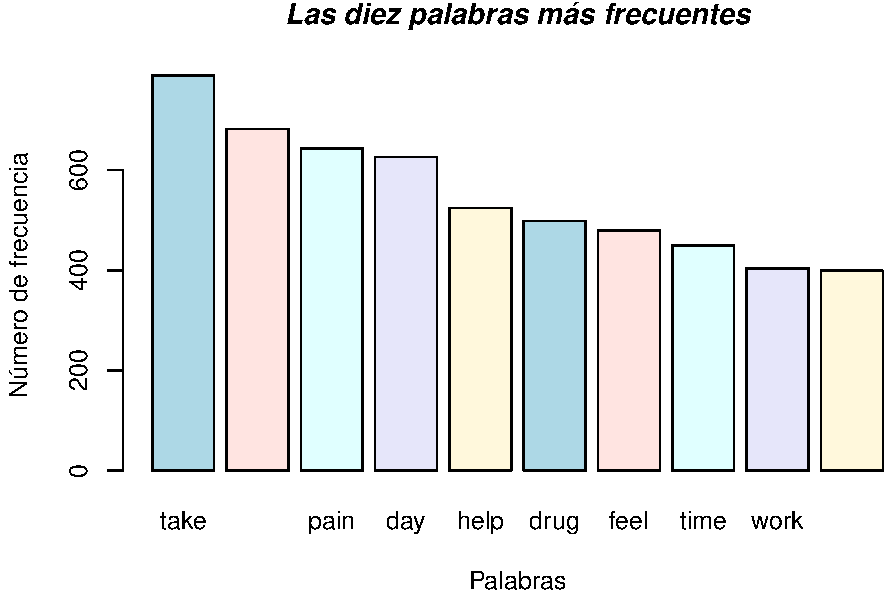
\includegraphics{practica_files/figure-latex/unnamed-chunk-33-1.pdf}


\end{document}
